\section{Evaluation}\label{sec:evaluation}

\subsection{Metrics}

To evaluate the performance of the models two metrics are utilized. The first one is the Levenshtein distance, also known as edit distance. The edit distance as depicted by Fig.~\ref{fig_edit_distance} calculates how many changes among insertions, deletions and substitutions are necessary to transform one string into another \cite{rice_edit_dist}. In this work all changes are weighted the same. The second metric is accuracy, which considers a prediction correct only if all characters match the label characters in the correct position. Originally \cite{icfhr_competition} considers from TOP-1 to TOP-3 submissions in case of accuracy, however this work considers only the TOP-1 network output. For the final results of the trained models in this section only accuracy is displayed since it is a harder metric and the only one which can be compared with the baseline results. 

\begin{figure}[t]
%\centerline{\epsfig{figure=figure,width=40mm}}
\centerline{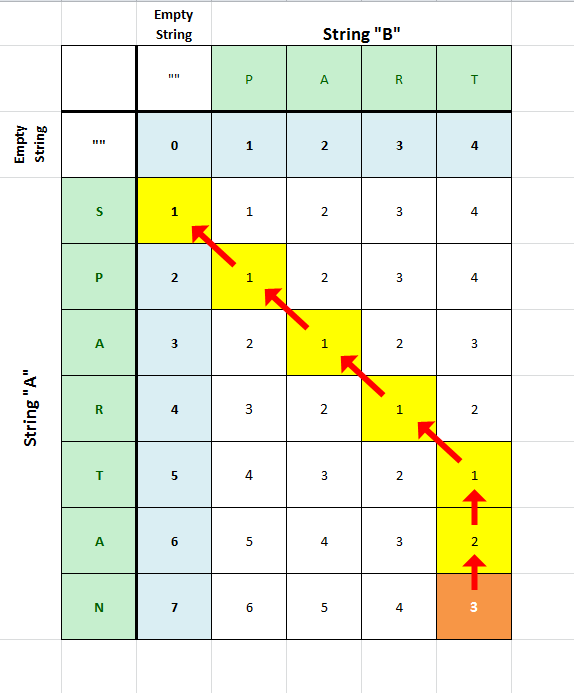
\includegraphics[width=40mm]{images/edit_distance}}
\caption{{\it Example of edit distance for words "part" and "spartan" by \cite{rice_edit_dist}.}}  
\label{fig_edit_distance}
\end{figure}

\subsection{Model performance}

The implemented model is similar to the one proposed by Zhan et al. \cite{zhan2017}, therefore its results are used as a reference of what can be achieved with an architecture using CNN + RNN-CTC. For each of the provided datasets, the model is trained for 100 epochs with Adam as optimizer, learning rate of \num{1e-04} and batch size equal to 16. The provided sets are already separated into training and test data, thus the training data was split further into 80\% of it for training and 20\% for validation. Table \ref{table_zhan_interpretation} summarizes the comparison between the base line and the used model. In each case of this comparison models were trained and tested only with data of the referenced dataset. 

\begin{table}
\caption{\label{table_zhan_interpretation} {\it Overall comparison between implementations.}}
\vspace{2mm}
\centerline{
\begin{tabular}{*{4}{|c}|}
\hline
Methods & 
CAR-A &
CAR-B & 
CVL\\
\hline \hline 
Zhan el al. 2017 & 0.8975 & 0.9114 & 0.2707 \\
Our "interpretation" & 0.9014 & 0.9084 & 0.2550 \\
\hline
\end{tabular}}
\end{table}

Given the fact that the model is able to perform well on CAR-A and CAR-B, experiments with cross-validation with data from different sets are made to evaluate if the reason for poor performance on CVL is the architecture or the model. Table \ref{table_different_sets} contains the results for models which were trained with datasets on the first line and tested against datasets on the first column. Considering only CAR-A and CAR-B, the best results are obtained by training and testing with data within a same set. The more interesting results are for CVL tests, as it has the worst performance when using its own training set and receives big performance improvements achieving almost 60\% if tested on a model which was trained exclusively with CAR-B data.  

\begin{table}
\caption{\label{table_different_sets} {\it Performance on different sets.}}
\vspace{2mm}
\centerline{
\begin{tabular}{*{4}{|c}|}
\hline
\backslashbox{Tested}{Trained} & 
CAR-A &
CAR-B & 
CVL\\
\hline \hline 
CAR-A & \textbf{0.9014} & 0.7315 & 0.002 \\
CAR-B & 0.8434 & \textbf{0.9084} & 0.006 \\
CVL & 0.3019 & \textbf{0.5804} & 0.2550 \\
\hline
\end{tabular}}
\end{table}

A further idea to improve the CVL performance follows the principle "more data is always better". As observed in the previous experiments as well as for reasons discussed in the data analysis in section \ref{introduction}, the CVL test data is not represented well by its training data, especially regarding the small amount of different string labels. The idea is therefore to adopt the whole training data of CAR-A plus CAR-B to train the model from scratch and additionally fine tune it on CVL. Taken into account from the previous experiments that the architecture is able to generalize well and to maximize the amount of training data, no validation data is used in these experiments. Apart from the lacking train-validation split, all the parameters remain the same. For fine tuning, all weights are trained for extra 20 epochs exclusively on CVL. 

The model trained on CAR-A+CAR-B without CVL data surpasses both the performances of models trained exclusively on these sets as well as the previously best CVL performance. By fine tuning the model on CVL however, the CVL test performance achieved almost 76\%, which compared to the results in \cite{icfhr_competition} means a second best CVL performance losing only to BeiJing et al. \cite{icfhr_competition}. 

\begin{table}
\caption{\label{table_fine_tuning} {\it Performance using more than one set + fine tuning.}}
\vspace{2mm}
\centerline{
\begin{tabular}{*{3}{|c}|}
\hline
\backslashbox{Tested}{Trained} & 
CAR-A + CAR-B &
CVL (fine tuning)\\
\hline \hline 
CAR-A & \textbf{0.9127} & 0.0565 \\
CAR-B & \textbf{0.9408} & 0.4733 \\
CVL & 0.5913 & \textbf{0.7579} \\
\hline
\end{tabular}}
\end{table}

\subsection{Error cases}

In order to have a better understanding of the mistakes the network makes, some of the errors during test are collected. Most of the errors fall into four classes. The first class is represented by Fig.~\ref{fig_error1}, in which the left border is misclassified as the digit "1", resulting in a prediction "175" versus label "75". Right borders can also be misclassified. A second class is as depicted by Fig.~\ref{fig_error2}, in which the digits cannot be easily classified correctly even by humans. In this case the network predicts "400" for a label "500". The third class of identified errors is illustrated by Fig.~\ref{fig_error3}. Due to the fact that the pictures do not include exclusively digits, symbols such as commas can be confused with the digit "1", despite the training to classify all strange symbols as "blank". The last error class is pictured by Fig.~\ref{fig_error4}. Given the CNN output, the input picture is divided in 15 parts to be classified by the RNN. A problem also occurs thereby if irrelevant symbols occupy too much space in a way that a single digit is too small inside one of these parts. For the example the prediction was "381", which suggests that the digits "29" are merged during the feature extraction. 

\begin{figure}[t]
    \centering
  \subfloat[Border\label{fig_error1}]{%
       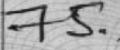
\includegraphics[width=0.2\linewidth]{images/error1}}
    \hfill
  \subfloat[Bad digits\label{fig_error2}]{%
        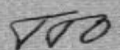
\includegraphics[width=0.2\linewidth]{images/error2}}
    \hfill
  \subfloat[Symbols\label{fig_error3}]{%
        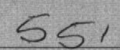
\includegraphics[width=0.2\linewidth]{images/error3}}
    \hfill
  \subfloat[Receptive field\label{fig_error4}]{%
        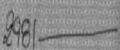
\includegraphics[width=0.2\linewidth]{images/error4}} \\
  \caption{{\it Examples of test errors}}
  \label{fig_methods} 
\end{figure}

Most of these errors can be probably avoided by investing more time into preprocessing the images, which is neglected in this work in favor of an end-to-end approach. Any extra preprocessing for such images requires feature engineering to remove irrelevant symbols by for example, searching for contours which are more likely to belong to digits as in Fig.~\ref{fig_preproc}. As a consequence the deep learning model would require less effort and complexity.  

\begin{figure}[t]
%\centerline{\epsfig{figure=figure,width=40mm}}
\centerline{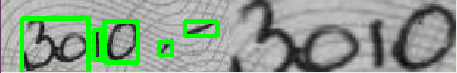
\includegraphics[width=40mm]{images/preproc}}
\caption{{\it Digit contour detection}.}  
\label{fig_preproc}
\end{figure}

\section{Lessons learned}

Of the many lessons learned during the development of this work, the most important is to recognize when overfitting is happening. Divergences between training and validation performance tend to happen but if they are too big a thoroughly analysis of the possible causes is necessary. Data augmentation and regularization methods do help but are not enough to overcome highly divergent performances, which are more likely caused by a wrong approach. Models for more complex tasks have so many parameters that is easy for them to memorize the training set completely without any generalization capability given enough epochs. 

A second lesson is to analyze carefully which type of information is passed to the LSTM input gates. Just reshaping tensors output by the CNN to fit the LSTM input shape without any reasonable criteria does not deliver any valuable results. At first it is not clear what to use as input in the presented problem since the sequence aspect is not instantly recognized as in problems which have for example image sequences as input or text sentences. Following the intuition of splitting the classification along the image width dimension, the LSTM time steps must also match this idea for learning effectively. 

\section{Conclusions}

This paper has described a novel approach for doing wonderful stuff such as ...
